\documentclass[10pt]{article}
\usepackage[cp1251]{inputenc}
\usepackage[english]{babel}
\usepackage{graphicx}
\usepackage[mag=1000,a4paper,left=2.2cm,right=3.0cm,top=3.0cm,bottom=3.0cm]{geometry}
\usepackage{enumerate}

\usepackage{latexsym, amsgen, amsmath, amstext, amsbsy, amsopn, amsfonts, amsthm, amssymb, amscd}
\usepackage{mathtext}
\usepackage{mathrsfs}

\title{Advanced Robotics}
\author{Melnikov E.\,R., Markeeva L.\,B., Usvyatsov M.\,R.}
\usepackage[cp1251]{inputenc}
\usepackage[normalem]{ulem}
\usepackage{indentfirst}
\usepackage{grffile}
\usepackage{epstopdf}
\usepackage{makeidx}
\usepackage{verbatim}
\usepackage{tikz}
\usepackage{ulem}
\usetikzlibrary{arrows}
\usetikzlibrary{shapes}
\usetikzlibrary{positioning}
\usetikzlibrary{calc}
\usepackage{caption}
\usepackage{hyperref}
\graphicspath{{images/}}

\frenchspacing
\parindent=0.6cm
\parskip=2pt
\mathsurround=1pt

\sloppy
\newtheorem{df}{Definition}
\newtheorem{stmt}{Statement}

\newtheorem{notice}{Notice}
\newtheorem{theo}{Theorem}

\def\proof{{\indent Proof.}}


\newcommand{\itemi}[1]{\item \emph{#1} }

\begin{document}
	\maketitle
	\section{Part 1}
		\subsection{Problem 1}
			\begin{figure}[h!]
				\center{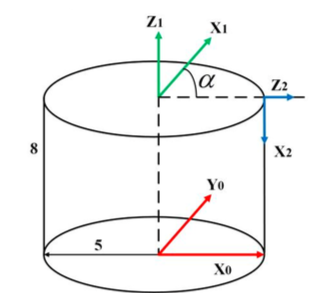
\includegraphics[width=0.8\textwidth]{1}}
				\caption{Problem 1 description}
				\label{fig:modules}
			\end{figure}
			
			\begin{enumerate}
				\item
					$^0_1R$ =
					$\left(
						\begin{tabular}{c c c}
							cos($\alpha$) & sin($\alpha$) & 0\\
							-sin($\alpha$) & cos($\alpha$) & 0\\
							0 & 0 & 1
						\end{tabular}
					\right)$
					
					$^0P$ = 
					$\left(
						\begin{tabular}{c}
							0\\
							0\\
							8
						\end{tabular}
					\right)$
					
					Thus $^0_1T$ = 
					$\left(
						\begin{tabular}{c c c c}
							cos($\alpha$) & sin($\alpha$) & 0 & 0\\
							-sin($\alpha$) & cos($\alpha$) & 0 & 0\\
							0 & 0 & 1 & 8\\
							0 & 0 & 0 & 1
						\end{tabular}
					\right)$
				\item
					$^2_1R$ =
					$\left(
						\begin{tabular}{c c c}
							cos($\alpha$) & sin($\alpha$) & 0\\
							-sin($\alpha$) & cos($\alpha$) & 0\\
							0 & 0 & 1
						\end{tabular}
					\right)$
					$\cdot$
					$\left(
						\begin{tabular}{c c c}
							0 & 0 & 1\\
							0 & 1 & 0\\
							-1 & 0 & 0
						\end{tabular}
					\right)$ =
					$\left(
						\begin{tabular}{c c c}
							0 & sin($\alpha$) & cos($\alpha$)\\
							0 & cos($\alpha$ & -sin($\alpha$)\\
							-1 & 0 & 0
						\end{tabular}
					\right)$
					
					We know, that $^A_BR = (^B_AR)^T$, thus $^1_2R$ =
					$\left(
						\begin{tabular}{c c c}
							0 & sin($\alpha$) & cos($\alpha$)\\
							0 & cos($\alpha$ & -sin($\alpha$)\\
							-1 & 0 & 0
						\end{tabular}
					\right)^T$ =
					$\left(
						\begin{tabular}{c c c}
							0 & 0 & -1\\
							sin($\alpha$) & cos($\alpha$) &0\\
							cos($\alpha$) &  -sin($\alpha$) & 0
						\end{tabular}
					\right)$
					
					$^1P$ = 
					$\left(
						\begin{tabular}{c}
							5$\cdot cos(\alpha)$\\
							-5$\cdot sin(\alpha)$\\
							0
						\end{tabular}
					\right)$
					
					Thus $^1_2T$ = 
					$\left(
						\begin{tabular}{c c c c}
							0 & 0 & -1 & 5$\cdot cos(\alpha)$\\
							sin($\alpha$) & cos($\alpha$) & 0 & -5$\cdot sin(\alpha)$\\
							cos($\alpha$) &  -sin($\alpha$) & 0 & 0\\
							0 & 0 & 0 & 1
						\end{tabular}
					\right)$
			\end{enumerate}

		\subsection{Problem 2}
			\begin{figure}[h!]
				\center{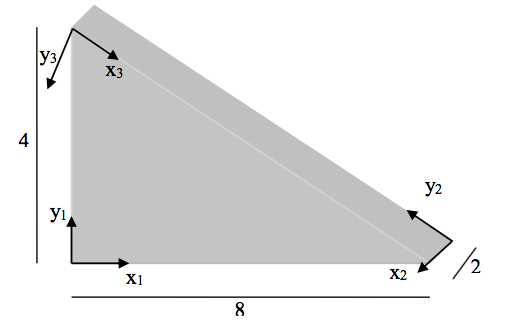
\includegraphics[width=0.8\textwidth]{2}}
				\caption{Problem 2 description}
				\label{fig:modules}
			\end{figure}

			\begin{enumerate}
				\item
					Let us define $\alpha$ = arctg(0.5)
					
					$^2_1R$ =
					$\left(
						\begin{tabular}{c c c}
							cos($\alpha$) & -sin($\alpha$) & 0\\
							sin($\alpha$) & cos($\alpha$) & 0\\
							0 & 0 & 1
						\end{tabular}
					\right)$
					$\cdot$
					$\left(
						\begin{tabular}{c c c}
							0 & 0 & -1\\
							0 & 1 & 0\\
							1 & 0 & 0
						\end{tabular}
					\right)$ =
					$\left(
						\begin{tabular}{c c c}
							0 & -sin($\alpha$) & -cos($\alpha$)\\
							0 & cos($\alpha$) & -sin($\alpha$)\\
							1 & 0 & 0
						\end{tabular}
					\right)$
					
					$^2P$ = 
					$\left(
						\begin{tabular}{c}
							2\\
							8$\cdot cos(\alpha)$\\
							8$\cdot sin(\alpha)$
						\end{tabular}
					\right)$
					
					Thus $^1_2T$ = 
					$\left(
						\begin{tabular}{c c c c}
							0 & -sin($\alpha$) & -cos($\alpha$) & 2\\
							0 & cos($\alpha$) & -sin($\alpha$) & 8$\cdot cos(\alpha)$\\
							1 & 0 & 0 & 8$\cdot sin(\alpha)$\\
							0 & 0 & 0 & 1
						\end{tabular}
					\right)$
				\item
					$^3_2R$ =
					$\left(
						\begin{tabular}{c c c}
							0 & 1 & 0\\
							-1 & 0 & 0\\
							0 & 0 & 1
						\end{tabular}
					\right)$
					$\cdot$
					$\left(
						\begin{tabular}{c c c}
							1 & 0 & 0\\
							0 & 0 & -1\\
							0 & 1 & 0
						\end{tabular}
					\right)$ =
					$\left(
						\begin{tabular}{c c c}
							0 & 0 & -1\\
							-1 & 0 & 0\\
							0 & 1 & 0
						\end{tabular}
					\right)$
					
					$^3P$ = 
					$\left(
						\begin{tabular}{c}
							2\\
							0\\
							4$\sqrt{5}$
						\end{tabular}
					\right)$
					
					Thus $^3_2T$ = 
					$\left(
						\begin{tabular}{c c c c}
							0 & 0 & -1 & 2\\
							-1 & 0 & 0 & 0\\
							0 & 1 & 0 & 4$\sqrt{5}$\\
							0 & 0 & 0 & 1
						\end{tabular}
					\right)$
				\item
					$^3_1R$ =
					$\left(
						\begin{tabular}{c c c}
							1 & 0 & 0\\
							0 & -1 & 0\\
							0 & 0 & -1
						\end{tabular}
					\right)$
					$\cdot$
					$\left(
						\begin{tabular}{c c c}
							$\dfrac{\sqrt{2}}{2}$ & -$\dfrac{\sqrt{2}}{2}$ & 0\\
							$\dfrac{\sqrt{2}}{2}$ & $\dfrac{\sqrt{2}}{2}$ & 0\\
							0 & 0 & 1
						\end{tabular}
					\right)$ =
					$\left(
						\begin{tabular}{c c c}
							$\dfrac{\sqrt{2}}{2}$ & -$\dfrac{\sqrt{2}}{2}$ & 0\\
							-$\dfrac{\sqrt{2}}{2}$ & -$\dfrac{\sqrt{2}}{2}$ & 0\\
							0 & 0 & -1
						\end{tabular}
					\right)$
					
					$^3P$ = 
					$\left(
						\begin{tabular}{c}
							4$\cdot sin(\alpha)$\\
							8$\cdot sin(\alpha)$\\
							0
						\end{tabular}
					\right)$
					
					Thus $^3_1T$ = 
					$\left(
						\begin{tabular}{c c c c}
							$\dfrac{\sqrt{2}}{2}$ & -$\dfrac{\sqrt{2}}{2}$ & 0 & 4$\cdot sin(\alpha)$\\
							-$\dfrac{\sqrt{2}}{2}$ & -$\dfrac{\sqrt{2}}{2}$ & 0 & 8$\cdot sin(\alpha)$\\
							0 & 0 & -1 & 0\\
							0 & 0 & 0 & 1
						\end{tabular}
					\right)$
				\item
					We know, that $^A_BT$ =
					$\left(
						\begin{tabular}{c c c | c}
							& $^A_BR$ & & $^AP$\\
							0 & 0 & 0 & 1
						\end{tabular}
					\right)$
					
					Furthermore, $^B_AT$ =
					$\left(
						\begin{tabular}{c c c | c}
							& $^B_AR$ & & $ - ^B_AR \cdot ^AP$\\
							0 & 0 & 0 & 1
						\end{tabular}
					\right)$
					
					Hence,  $^1_3T$ = 
					$\left(
						\begin{tabular}{c c c c}
							$\dfrac{\sqrt{2}}{2}$ & -$\dfrac{\sqrt{2}}{2}$ & 0 & -$2 \sqrt{2} \cdot sin(\alpha)$\\
							-$\dfrac{\sqrt{2}}{2}$ & -$\dfrac{\sqrt{2}}{2}$ & 0 & -$4 \sqrt{2} \cdot sin(\alpha)$\\
							0 & 0 & -1 & 0\\
							0 & 0 & 0 & 1
						\end{tabular}
					\right)$
			\end{enumerate}
\end{document}